\documentclass[10pt,a4paper]{article}
\usepackage[T1]{fontenc}
\usepackage{lmodern,textcomp}
\usepackage[margin=2.4cm]{geometry}
\usepackage{amsmath,amssymb,amsthm}
\usepackage{graphicx,booktabs,array,float}
\usepackage[hidelinks]{hyperref}
\usepackage{microtype}
\setlength{\parskip}{3pt}
\newtheorem{proposition}{Proposition}
\newtheorem{definition}{Definition}
\renewcommand{\arraystretch}{1.1}
\begin{document}
\title{\bfseries Revenue Forecaster: a Sequential-Flow Model for Financial Lead Pingtrees\\[2pt]\large Forecasting revenue and choosing the order of buyers}
\author{Humbert Pou Plana}
\date{November 2026}
\maketitle
\begin{abstract}
Lead-generation businesses in consumer finance sell each lead through a \emph{pingtree}: an ordered list of buyers who are offered the lead in sequence until one accepts. We present a forecasting model that turns a client's lead volume into expected monthly revenue by propagating leads through a pingtree built from the buyers' observed acceptance rates and earnings per lead (EPL). We prove that ordering buyers by decreasing EPL maximises expected revenue when acceptances are independent and offers are free, quantify the forecast on anonymised data for January--February 2026, and reconcile it with realised revenue. The unadjusted flow, in which every buyer is offered every leftover lead, gives 115,371\,\texteuro{} per 100{,}000 leads, but this is a ceiling: buyers are only queried for a fraction of leads. Adjusting for each buyer's observed reach gives 16,300\,\texteuro{} and reproduces realised monthly revenue (in-sample ratio 93\%; walk-forward mean absolute percentage error 17.6\%). We also show how concentration, diminishing returns, sample-size filters and Monte Carlo uncertainty shape the result, and where the independence assumption is likely to fail.
\end{abstract}

\section{Introduction}
A \emph{pingtree} (or waterfall) sells a lead to the first buyer in an ordered list that accepts it. The order matters because every lead accepted early is no longer available to later buyers. A seller that holds a pool of leads therefore needs two answers: how much revenue will the pool generate, and in which order should buyers be called. This paper describes a small forecasting tool, the \emph{Revenue Forecaster}, that answers both from historical acceptance and revenue statistics, and documents the mathematics behind it.

The contribution is deliberately modest. We give (i) a clean sequential-flow model, (ii) a short proof that EPL-descending order is optimal under stated assumptions, (iii) an empirical illustration on anonymised data, and (iv) an honest list of the assumptions that real deployments will violate.

\section{Model}
Let $N$ be the number of leads entering the pingtree and let buyers be indexed by their position $i=1,\dots,n$. For buyer $i$ let $a_i\in[0,1]$ be the \emph{acceptance rate} (accepted leads divided by leads offered) and $e_i\ge 0$ the \emph{earnings per lead} (revenue divided by accepted leads). The number of leads reaching position $i$ is
\begin{equation}
 L_i = N\prod_{j<i}(1-a_j),
\end{equation}
so buyer $i$ accepts $A_i=a_iL_i$ leads and generates revenue $A_ie_i$. Expected total revenue is
\begin{equation}
 R(\pi)=N\sum_{i=1}^{n} a_i e_i \prod_{j<i}(1-a_j),
\end{equation}
where $\pi$ denotes the ordering. The share of leads placed is $1-\prod_i(1-a_i)$, which does not depend on the order.

\begin{proposition}\label{prop:order}
Assume acceptances are independent across buyers, an offer to a buyer costs nothing, and $a_i,e_i$ do not depend on position. Then $R(\pi)$ is maximised by ordering buyers by non-increasing $e_i$.
\end{proposition}
\begin{proof}
Consider two adjacent buyers at positions $k$ and $k+1$ with parameters $(a,e)$ and $(a',e')$, and let $\Pi=\prod_{j<k}(1-a_j)$. Their contribution to $R/N$ in the order $(a,e),(a',e')$ is $\Pi\,[\,ae+(1-a)a'e'\,]$. Swapping them gives $\Pi\,[\,a'e'+(1-a')ae\,]$. The difference is
\begin{equation}
 \Pi\,[\,ae+(1-a)a'e'-a'e'-(1-a')ae\,]=\Pi\,aa'(e-e').
\end{equation}
The leads that continue past both buyers are the same in either order, so later terms are unchanged. Hence swapping adjacent buyers never lowers revenue when the one with the higher EPL is moved forward. Any ordering can be sorted into EPL-descending order by adjacent swaps, each of which weakly increases $R$. \qedhere
\end{proof}
The result is a local index rule in the spirit of sequential search problems \cite{weitzman}. It breaks down when offers are costly, when buyers have monthly caps, or when acceptance depends on position, which we discuss in Section~\ref{sec:limits}. The tool includes a \emph{position penalty} $\rho\in[0,1]$ that scales the acceptance of the buyer at position $i$ by $1-\rho\,(i-1)/(n-1)$ to probe the last case.

\subsection{Reach adjustment}\label{sec:reach}
The flow above implicitly offers every unplaced lead to every buyer. In practice a buyer only receives requests for a subset of leads (eligibility rules, caps, product fit), and its observed acceptance rate is measured on that subset. Let $q_i=\min(1,R_i/N_{\mathrm{ref}})$ be the share of leads for which buyer $i$ is queried, where $R_i$ is the buyer's requests and $N_{\mathrm{ref}}$ is the lead volume (the largest request volume in each month, summed over the aggregated months). Replacing $a_i$ by $q_ia_i$ in the flow gives the \emph{reach-adjusted} forecast. Proposition~\ref{prop:order} still applies with $q_ia_i$ as the effective acceptance, so EPL-descending order remains optimal. With $q_i=1$ for all buyers we recover the \emph{full-reach} forecast, which is an upper bound.

\subsection{Uncertainty}
Monthly acceptance and EPL fluctuate. For each buyer we estimate the coefficient of variation of both quantities over the monthly observations from 2025-09 onwards (bounded between 3\% and 80\%, with a default of 20\% when fewer than two months exist) and draw multiplicative log-normal noise with unit mean. Accepted leads at each position are drawn from a normal approximation to the binomial. We report the 10th, 50th and 90th percentiles of 2{,}000 simulations (fixed seed).

\section{Data and calibration}
The reference data are anonymised sources: for each of 42 buyers and 14 months (January 2025 to February 2026), the number of requests, accepted leads, sales and revenue; buyer identifiers are pseudonymised. The dataset and its data dictionary ship with the repository. Buyer statistics for the forecast are pooled over 2026-01 and 2026-02, so $a_i$ is total accepted over total requests and $e_i$ is total revenue over total accepted; coefficients of variation for the Monte Carlo use the six monthly observations from 2025-09. Both windows are parameters of a single configuration file used by the code, the tests and this paper. Buyers with no revenue, or with fewer than 50 accepted leads, are excluded; this leaves 40 eligible buyers, of which the top 20 by EPL form the pingtree. Buyers are labelled P1--P20 by position. Some buyers are paid per accepted lead rather than per sale, so their conversion rate is not defined and is shown as unavailable in the tool.

\section{Results}
\subsection{Baseline forecast}
For $N=100{,}000$ leads per month and a 20-offer pingtree, the full-reach model forecasts 115,371\,\texteuro{} per month, or 1.15\,\texteuro{} per lead; this is the ceiling discussed in Section~\ref{sec:recon}. 33.0\% of leads are placed and the average EPL is 3.50\,\texteuro{}. Table~\ref{tab:tree} lists the pingtree and Figure~\ref{fig:flow} shows how leads are consumed along it.
\begin{table}[H]\centering\small
\caption{Forecast pingtree for 100{,}000 leads per month. Acc.\ is the acceptance rate in \%, EPL is in euros and revenue in euros.}\label{tab:tree}
\begin{tabular}{lrrrrrr}\toprule
Buyer & Leads in & Acc.\ (\%) & Accepted & EPL & Revenue & Share (\%)\\\midrule
P1 & 100,000 & 0.65 & 649 & 29.59 & 19,202 & 16.6\\
P2 & 99,351 & 0.65 & 645 & 17.31 & 11,171 & 9.7\\
P3 & 98,706 & 0.80 & 787 & 17.30 & 13,613 & 11.8\\
P4 & 97,919 & 1.70 & 1,666 & 6.22 & 10,366 & 9.0\\
P5 & 96,252 & 0.74 & 708 & 4.48 & 3,170 & 2.7\\
P6 & 95,544 & 1.00 & 960 & 3.88 & 3,721 & 3.2\\
P7 & 94,585 & 0.74 & 702 & 3.31 & 2,323 & 2.0\\
P8 & 93,883 & 0.04 & 34 & 3.14 & 107 & 0.1\\
P9 & 93,849 & 2.85 & 2,674 & 2.71 & 7,233 & 6.3\\
P10 & 91,175 & 0.13 & 114 & 2.70 & 308 & 0.3\\
P11 & 91,061 & 0.46 & 420 & 2.35 & 988 & 0.9\\
P12 & 90,641 & 2.88 & 2,613 & 2.04 & 5,322 & 4.6\\
P13 & 88,028 & 0.98 & 864 & 2.00 & 1,728 & 1.5\\
P14 & 87,164 & 10.38 & 9,049 & 1.98 & 17,933 & 15.5\\
P15 & 78,115 & 0.78 & 612 & 1.84 & 1,129 & 1.0\\
P16 & 77,503 & 2.06 & 1,595 & 1.77 & 2,828 & 2.5\\
P17 & 75,908 & 0.14 & 106 & 1.68 & 177 & 0.2\\
P18 & 75,802 & 11.01 & 8,345 & 1.60 & 13,346 & 11.6\\
P19 & 67,458 & 0.50 & 337 & 1.60 & 539 & 0.5\\
P20 & 67,120 & 0.18 & 119 & 1.43 & 169 & 0.1\\
\bottomrule\end{tabular}\end{table}
\begin{figure}[H]\centering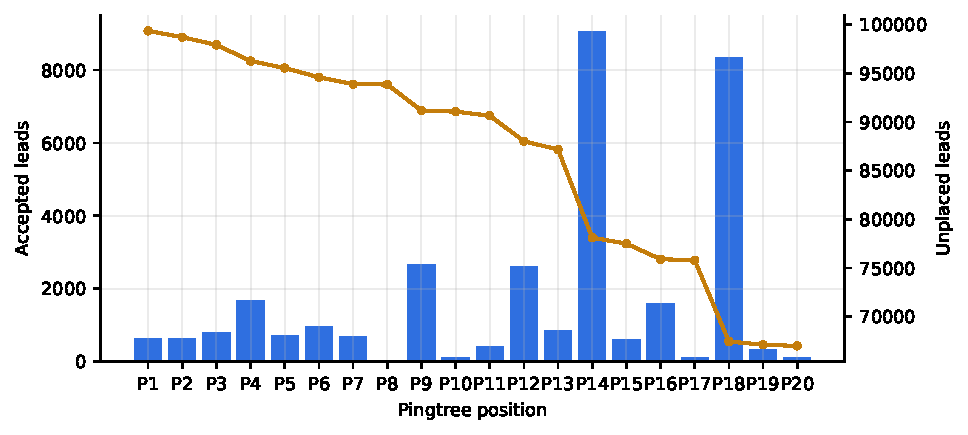
\includegraphics[width=0.92\linewidth]{fig/p1_flow.pdf}\caption{Leads accepted by each buyer (bars) and leads still unplaced after each position (line).}\label{fig:flow}\end{figure}

The first buyer sees every lead, but because acceptance rates are low (most below 10\%) the pool decays slowly, and about two thirds of leads are still unplaced after the twentieth buyer.

\subsection{Concentration and diminishing returns}
Revenue is concentrated: the top buyer produces 16.6\% of the total and the top three 38.1\%; the first 14 buyers reach 80\% of revenue (Herfindahl--Hirschman index 1,059). Figure~\ref{fig:rev} shows revenue by position. Adding offers has diminishing returns (Figure~\ref{fig:marg}): going from 15 to 20 offers adds 17,059\,\texteuro{} per month, and revenue with 10 offers is 38\% lower than with 20.
\begin{figure}[H]\centering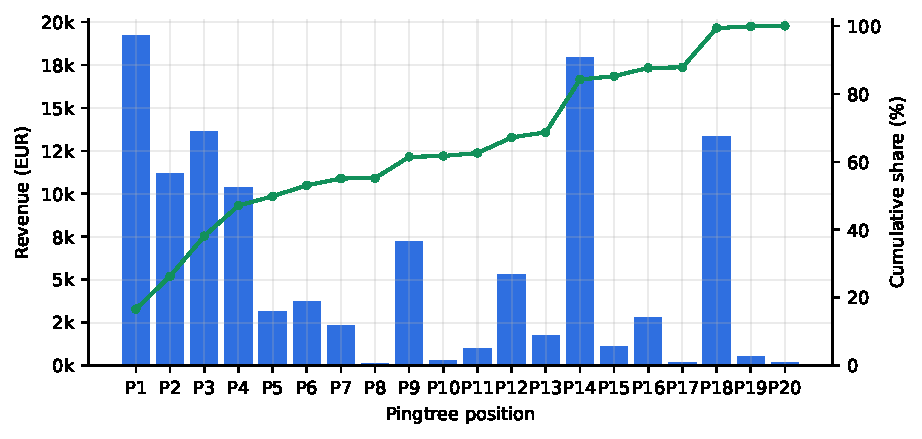
\includegraphics[width=0.92\linewidth]{fig/p1_rev.pdf}\caption{Forecast revenue by position (bars) and cumulative share of the total (line).}\label{fig:rev}\end{figure}

\begin{figure}[H]\centering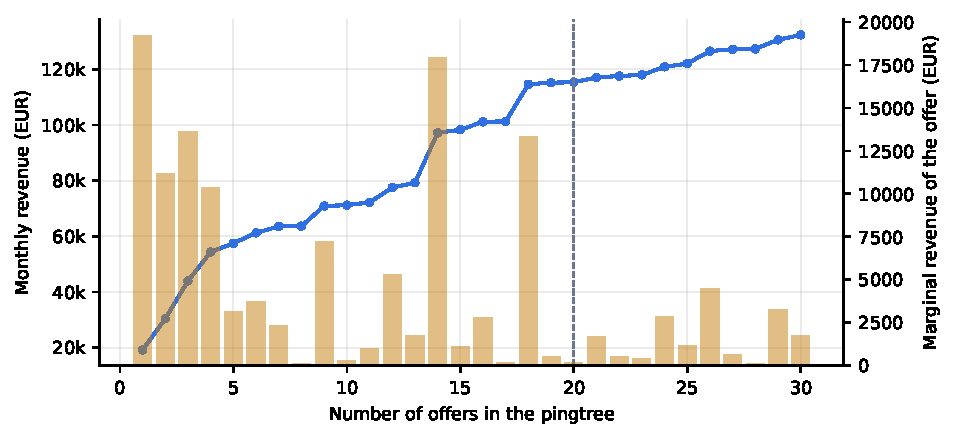
\includegraphics[width=0.92\linewidth]{fig/p1_marg.pdf}\caption{Total revenue as the number of offers grows (line) and marginal revenue of each added offer (bars).}\label{fig:marg}\end{figure}

\subsection{Does order matter?}
Figure~\ref{fig:order} compares the proposed order with alternatives for the same 20 buyers. Ordering by EPL gives 115,371\,\texteuro{}; ordering by acceptance rate gives 98,943\,\texteuro{}, by historical revenue 104,577\,\texteuro{}, and a random order averages 106,125\,\texteuro{}. The worst case, ascending EPL, yields 97,842\,\texteuro{}. EPL-descending order is therefore 9\% better than a random order, consistent with Proposition~\ref{prop:order}.
\begin{figure}[H]\centering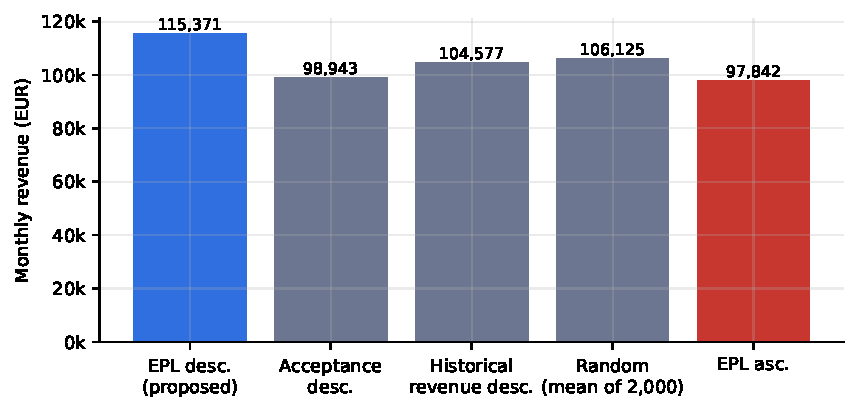
\includegraphics[width=0.8\linewidth]{fig/p1_order.pdf}\caption{Forecast revenue of the same 20 buyers under different ordering criteria.}\label{fig:order}\end{figure}

\subsection{Uncertainty and sensitivity}
The Monte Carlo simulation gives a median of 114,135\,\texteuro{} with a 10th--90th percentile range of 102,231\,\texteuro{} to 129,196\,\texteuro{} (Figure~\ref{fig:mc}). Figure~\ref{fig:sens} shows that a 10\% change in either acceptance or EPL moves the forecast by about 9--10\%, a 30\% position penalty costs 10\%, and cutting the pingtree to 10 offers costs 38\%.
\begin{figure}[H]\centering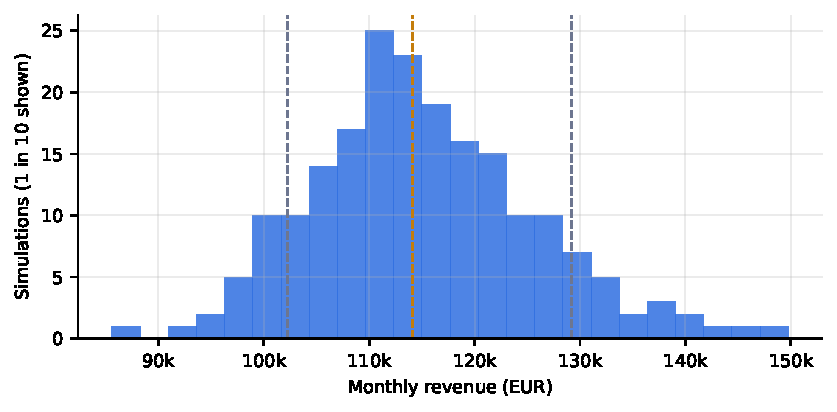
\includegraphics[width=0.8\linewidth]{fig/p1_mc.pdf}\caption{Distribution of monthly revenue over 2{,}000 simulations; dashed lines mark the 10th, 50th and 90th percentiles.}\label{fig:mc}\end{figure}

\begin{figure}[H]\centering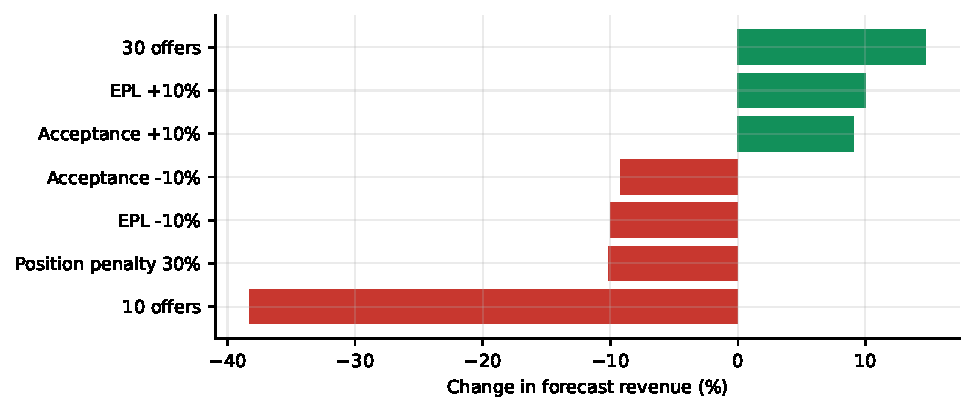
\includegraphics[width=0.8\linewidth]{fig/p1_sens.pdf}\caption{Sensitivity of the forecast to changes in assumptions.}\label{fig:sens}\end{figure}

\subsection{Sample-size filter and month-to-month variation}
Small samples are dangerous. Without any minimum on accepted leads the forecast rises to 4,500,000\,\texteuro{}, because a handful of buyers with very few accepted leads show an implausibly high EPL and move to the top of the tree. With a minimum of 50, 200 and 1{,}000 accepted leads the forecasts are 115,371\,\texteuro{}, 91,388\,\texteuro{} and 100,210\,\texteuro{}. The default of 50 is a compromise, not a recommendation: the right threshold should be chosen by cross-validating forecasts against realised revenue. Forecasts based on January alone and February alone are 107,246\,\texteuro{} and 90,022\,\texteuro{}, a spread that the Monte Carlo range only partly captures and that is a reminder that two months of data are a thin base.
\begin{figure}[H]\centering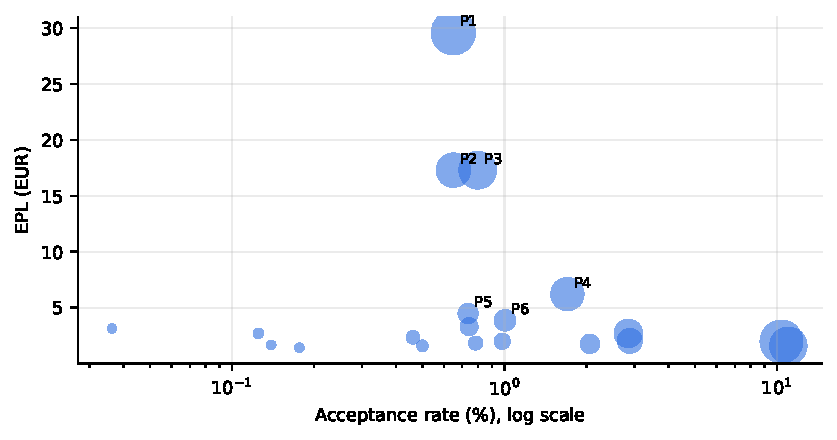
\includegraphics[width=0.78\linewidth]{fig/p1_bubble.pdf}\caption{EPL against acceptance rate for the 20 buyers. Bubble area is forecast revenue; the horizontal axis is logarithmic.}\label{fig:bubble}\end{figure}

\section{Reconciliation with realised revenue}\label{sec:recon}
The full-reach figure is an upper bound and should not be read as a prediction of what a pingtree earns today. To test this we use realised revenue, the sum of the revenue column over buyers, and the monthly lead volume $N_t$ (largest request volume of any buyer in month $t$). Month by month, the reach-adjusted flow fed with the same month's rates and ordered by requests (a proxy for the observed order) reaches on average 93\% of realised revenue (range 90\% to 96\%). A walk-forward backtest estimates rates on the previous 2 months, orders buyers by EPL, uses the realised $N_t$ and compares the forecast with realised revenue over 12 months: the mean absolute percentage error is 17.6\% (bias +6.0\%), against 18.8\% for a naive run-rate forecast, while the full-reach flow overstates realised revenue by a median factor of 5.1. For 100{,}000 leads the reach-adjusted forecast is 16,300\,\texteuro{} (P10--P90 13,632\,\texteuro{} to 19,339\,\texteuro{}), roughly 7.1 times lower than the ceiling.
\begin{table}[H]\centering\small
\caption{Walk-forward backtest. Forecasts use rates from the previous 2 months and the realised lead volume of the target month.}\label{tab:bt}
\begin{tabular}{lrrr}\toprule
Month & Realised (EUR) & Reach-adjusted (EUR) & Error (\%)\\\midrule
2025-03 & 527,489 & 351,982 & -33.3\\
2025-04 & 458,637 & 429,698 & -6.3\\
2025-05 & 478,520 & 505,009 & +5.5\\
2025-06 & 457,528 & 406,214 & -11.2\\
2025-07 & 502,494 & 491,269 & -2.2\\
2025-08 & 496,929 & 639,628 & +28.7\\
2025-09 & 480,207 & 557,136 & +16.0\\
2025-10 & 396,224 & 567,792 & +43.3\\
2025-11 & 324,293 & 430,259 & +32.7\\
2025-12 & 339,788 & 390,848 & +15.0\\
2026-01 & 349,751 & 296,710 & -15.2\\
2026-02 & 105,374 & 103,839 & -1.5\\
\bottomrule\end{tabular}\end{table}
\begin{figure}[H]\centering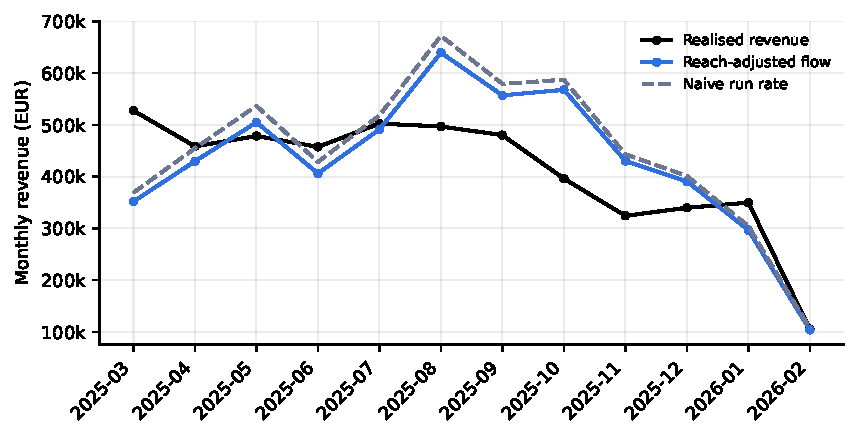
\includegraphics[width=0.85\linewidth]{fig/p1_backtest.pdf}\caption{Realised monthly revenue and walk-forward forecasts (reach-adjusted flow and naive run rate).}\label{fig:bt}\end{figure}

The reach-adjusted model is slightly better than a naive run rate, so it adds little accuracy at the aggregate level; its value is structural: it explains revenue by buyer and position and it is the right base for what-if questions such as changing the order or adding offers. Two caveats apply. The lead volume is an input, so the backtest does not test volume forecasting; and the observed order is only approximated.

\section{Limitations and extensions}\label{sec:limits}
\paragraph{Position-dependent acceptance.} Acceptance rates were measured in the positions buyers actually occupied. Buyers placed lower see leads already rejected by others, which may have lower quality, so their acceptance in a new tree could be smaller. The position-penalty parameter lets users test this, but the correct approach is to estimate acceptance by position from experiments.
\paragraph{Caps and costs.} Many buyers impose monthly caps. With caps the optimal order is no longer an index rule and a small optimisation problem must be solved. If pings have a cost, buyers with low acceptance and moderate EPL may not be worth calling.
\paragraph{Lead types.} The quality adjustments for lead types in the tool are editable hypotheses. They are not estimated from data and should be replaced by segment-level statistics.
\paragraph{Independence.} Acceptance decisions are modelled as independent. In practice buyers use similar eligibility rules, so a lead rejected by one is more likely to be rejected by another, which would make the forecast optimistic. The reach adjustment partly absorbs this effect, because it scales acceptance to the leads each buyer actually receives, but it does not model correlation between buyers.
\paragraph{Forecast, not guarantee.} The output is an expected value under stated assumptions, not a commitment.

\section{Conclusion}
A sequential-flow model with a simple ordering theorem is enough to build a transparent revenue forecaster for lead pingtrees. On anonymised data the full-reach forecast for 100{,}000 leads is 115,371\,\texteuro{} per month (Monte Carlo range 102,231\,\texteuro{} to 129,196\,\texteuro{}), a ceiling; the reach-adjusted forecast of 16,300\,\texteuro{} reconciles with realised revenue. The main practical risks are small samples, position effects and caps; each can be addressed with the extensions above.

\begin{thebibliography}{9}
\bibitem{weitzman} M.~L. Weitzman. Optimal search for the best alternative. \emph{Econometrica}, 47(3):641--654, 1979.
\bibitem{glasserman} P.~Glasserman. \emph{Monte Carlo Methods in Financial Engineering}. Springer, 2004.
\end{thebibliography}
\end{document}
